\section{Аналитическая часть}

\subsection{Анализ предметной области}\label{scene}

\textbf{Фитнес-клуб} -- это учреждение, оснащённое оборудованием для физических упражнений, предоставляющие услуги в области физической активности и здоровья~\cite{IHRSA2019, leonquismondo2020service}. 

\textbf{Главная цель} фитнес-клуба: обеспечение комфортных условий для физической активности клиентов, улучшении их здоровья и поддержании высокого уровня физической формы~\cite{IHRSA2019, leonquismondo2020service, bates2019health}.

\textbf{Основные функции} фитнес-клуба:
\begin{itemize}
	\item обеспечение тренировок и активного отдыха для клиентов;
	\item предоставление абонементов с различными условиями для доступа к услугам клуба;
	\item управление расписанием тренировок;
	\item учет посещений, тренировки и прогресса клиентов~\cite{bates2019health}.
\end{itemize}

\textbf{Клиенты} фитнес-клуба -- физические лица, которые заинтересованы в поддержании физической активности и улучшении здоровья. Например, люди, занимающиеся спортом для поддержания физической формы или проходящие реабилитацию для восстановление после травм~\cite{leonquismondo2020service, bates2019health}.

\textbf{Абонементы} являются основным способом доступа клиентов к услугам фитнес-клуба, и их типы определяются самим клубом в зависимости от потребностей и предпочтений клиентов. Например, могут быть предложены ежемесячные абонементы (предоставляющие доступ на один месяц) либо годовые абонементы (с выгодными условиями на длительный период)~\cite{bates2019health}.

Основными \textbf{сотрудниками} фитнес-клуба являются:
\begin{itemize}
	\item \textbf{администраторы}, которые управляют клиентской базой, занимаются продажей абонементов, отслеживанием посещаемости и предоставляют информацию о клубе.
	
	\item \textbf{тренеры} -- специалисты, которые проводят тренировки для клиентов~\cite{bates2019health}. 
\end{itemize}

\subsection{Формализация задачи}

Целью данной курсовой работы является разработка базы данных для хранения и обработки информации фитнес-клуба. 

Предметная область задачи охватывает деятельность фитнес-клуба, включая управление данными о клиентах (их личной информации, тренировках, истории посещений), тренерах (их расписаниях, специализациях) и организации тренировок, расписаний, а также систему учета абонементов и оплат. 

Цель создания базы данных -- автоматизировать процессы учета и повысить эффективность функционирования фитнес-клуба, а также улучшить обслуживание клиентов.

Для взаимодействия с базой данных фитнес-клуба необходимо разработать интерфейс, который обеспечит функциональный доступ к ключевым операциям системы в зависимости от роли пользователя.

Интерфейс должен предусматривать следующие возможности:
\begin{itemize}
	\item регистрация и авторизация пользователей;
	\item приобретение абонементов и управление ими;
	\item запись на тренировки и управление расписанием.
\end{itemize}

В рамках данной курсовой работы не рассматривается вопрос обеспечения конфиденциальности персональных данных пользователей и интеграции платежной системы:
\begin{itemize}
	\item все данные, включая контактные и учетные данные пользователей, будут храниться в базе данных без использования специализированных механизмов защиты конфиденциальности;
	\item не реализуется функциональность для работы с платежными системами и интеграция с внешними платёжными сервисами для обработки финансовых транзакций или хранения данных о платежах.
\end{itemize}

\newpage
\subsection{Формализация данных}

На рисунке~\ref{fig:er-chen} изображена диграмма сущность--связь в нотации Чена.

\begin{figure}[ht!]
	\begin{center}
		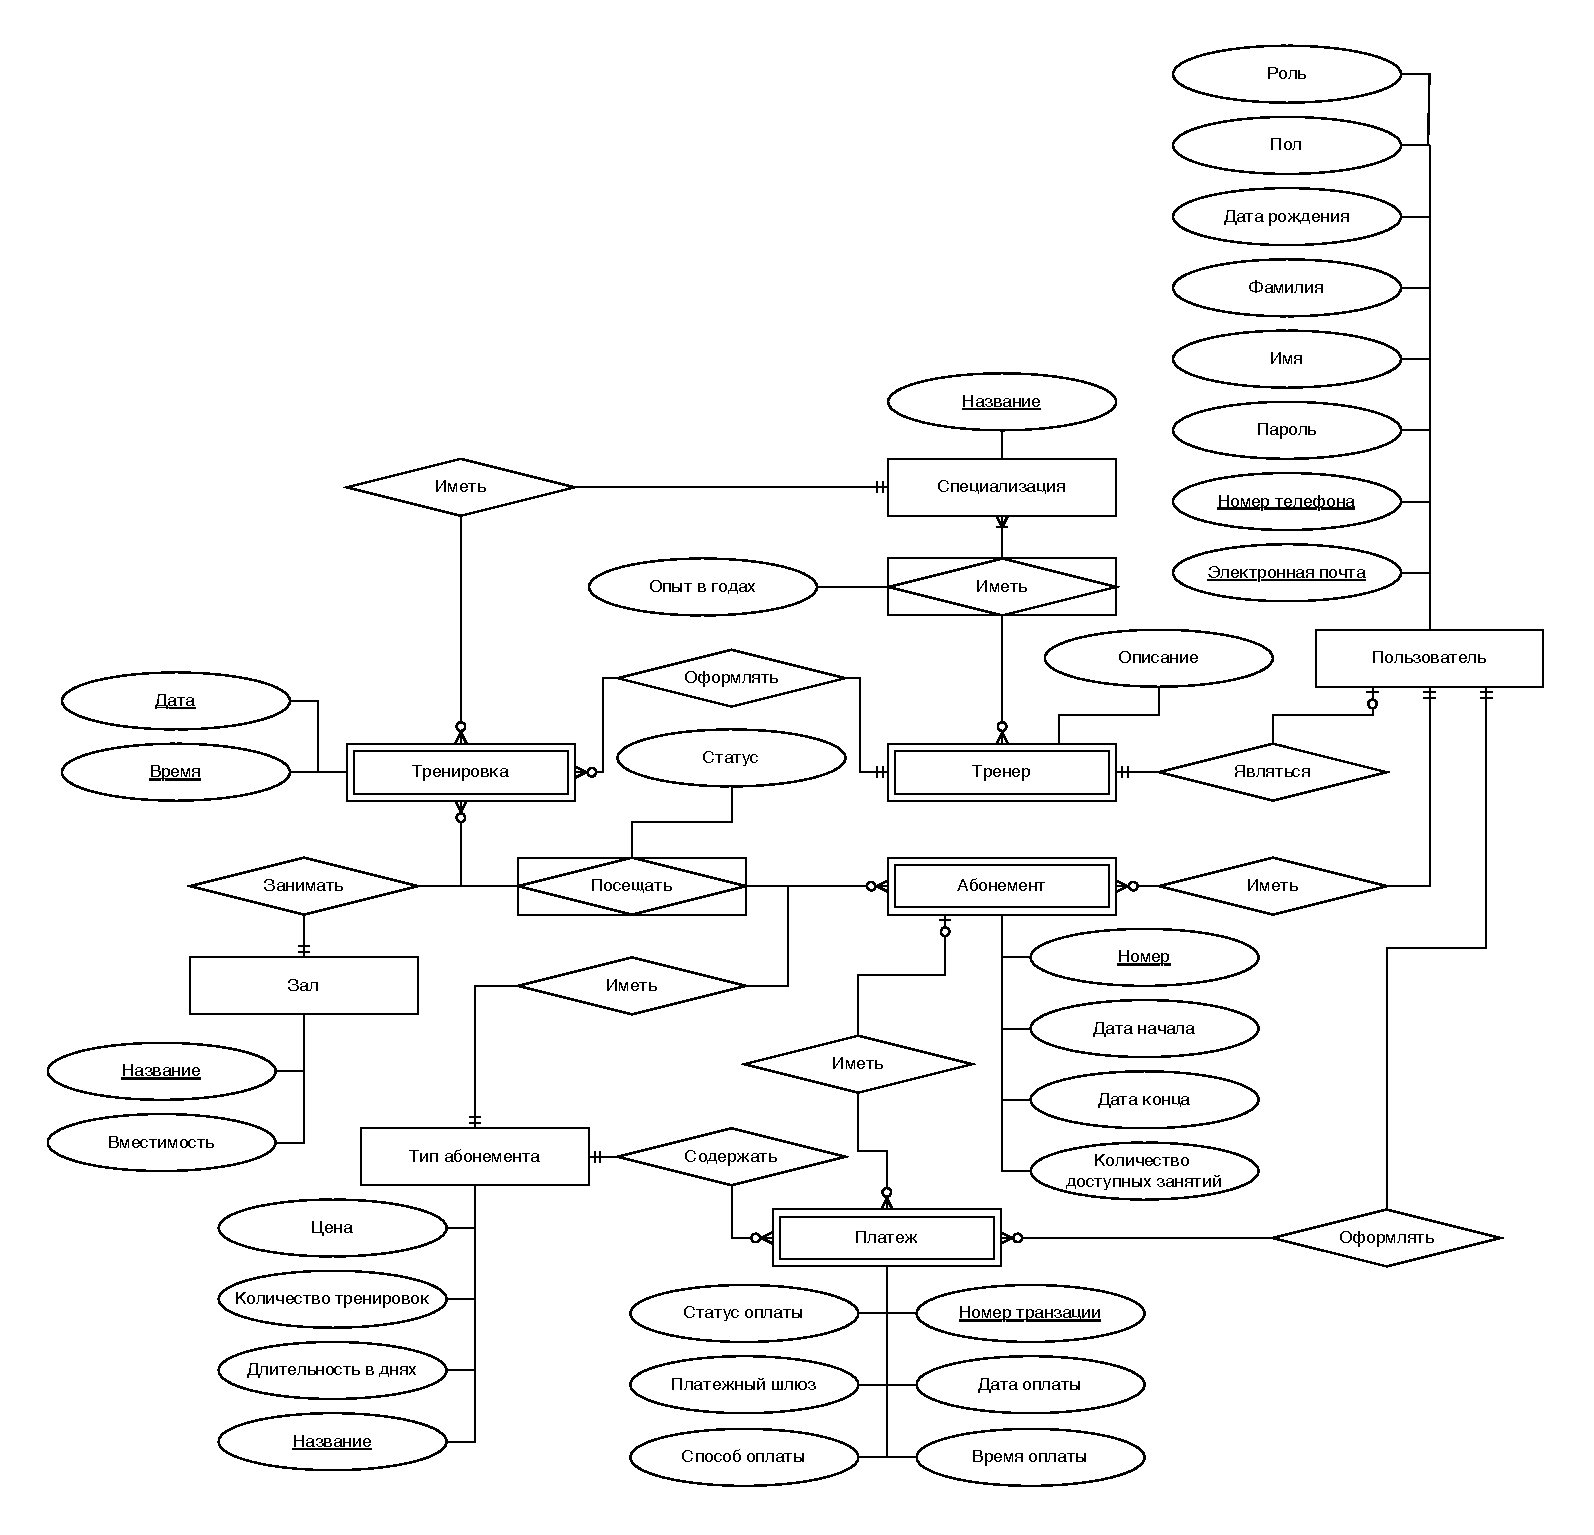
\includegraphics[scale=0.62]{./diag/er-chen.pdf}
	\end{center}
	\caption{ER-диаграмма фитнес-клуба в нотации Чена}
	\label{fig:er-chen}
\end{figure}

В базе данных для фитнес-клуба можно выделить следующие ключевые сущности.
\begin{enumerate}[label=\arabic*.]
	\item \textbf{Пользователь} -- основная сущность, представляющая всех участников системы: клиентов, тренеров и администраторов.

	\item \textbf{Роль пользователя} -- сущность, определяющая уровень доступа и права пользователя в системе.

	\item \textbf{Тренер} -- сущность, связанная с пользователем, имеющим соответствующую роль тренера.

	\item \textbf{Специализация} -- сущность, которая определяет специализацию и используется для описания тренировок и компетенций тренеров.

	\item \textbf{Тип абонемента} -- сущность, описывающая варианты абонементов, устанавливаемые фитнес-клубом.

	\item \textbf{Абонемент} -- сущность, отражающая приобретённый пользователем абонемент.

	\item \textbf{Заказ} и \textbf{позиция заказа} -- сущности, которые фиксируют процесс приобретения абонементов пользователями.

	\item \textbf{Платеж} -- сущность, отражающая факт оплаты заказа.

	\item \textbf{Зал} -- сущность, которая содержит информацию о помещениях для проведения тренировок.

	\item \textbf{Тренировка} --  сущность, представляющая собой запланированное мероприятие -- тренировку.

	\item \textbf{Посещение} -- сущность, которая фиксирует факт участия клиента в конкретной тренировке.
\end{enumerate}

\subsection{Формализация пользователей и их прав доступа}

Взаимодействовать c базой данных будут четыре вида пользователей.

На рисунке~\ref{fig:use-case} приведена диаграмма вариантов использования базы данных.

\begin{figure}[ht!]
	\begin{center}
		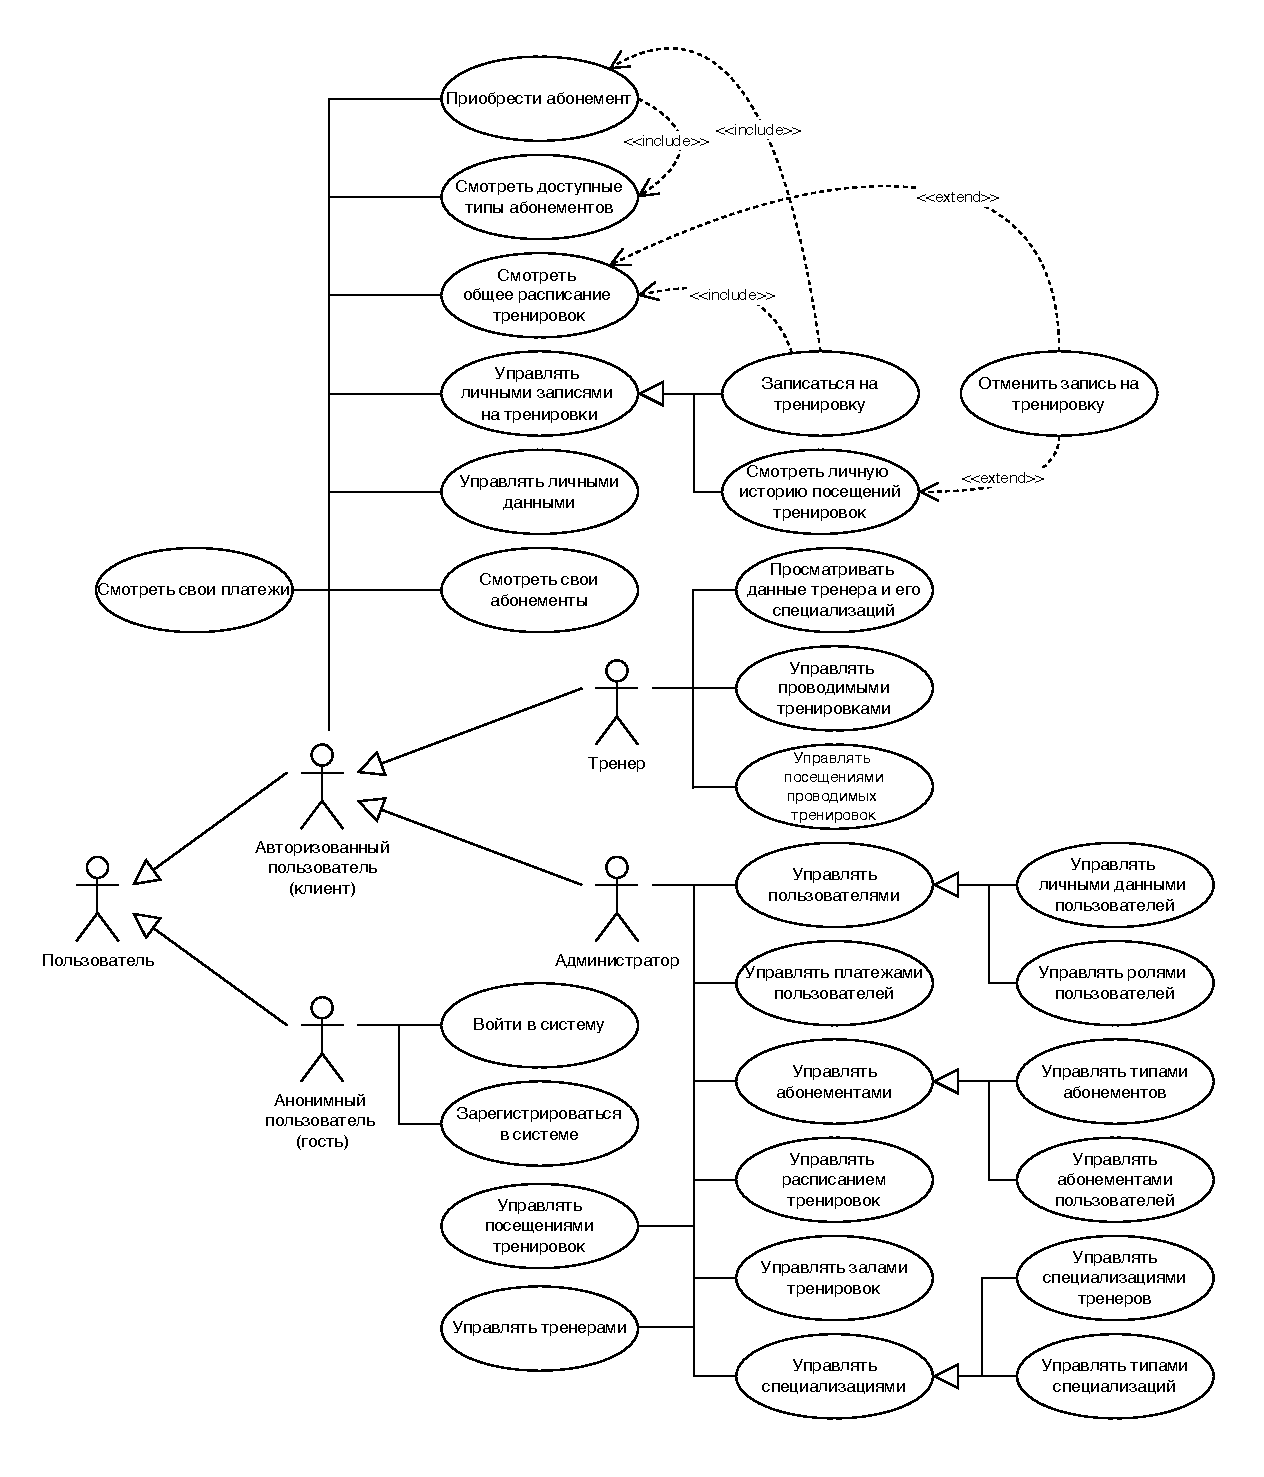
\includegraphics[scale=0.8]{./diag/use-case.pdf}
	\end{center}
	\caption{Диаграмма вариантов использования базы данных}
	\label{fig:use-case}
\end{figure}

\textbf{Гость} -- анонимный пользователь, который может выполнять только определенные действия, такие как регистрация и вход в систему.

Авторизованные пользователи: 
\begin{enumerate}[label=---]
	\item \textbf{клиент} -- пользователь, который имеет минимальные права, ограниченные только возможностью взаимодействовать с данными, относящимися к его учетной записи и обслуживанию (например, заказами, абонементами и посещениями).
	
	\item \textbf{тренер} -- пользователь, имеющий права клиента, а также имеющий доступ к данным, связанным с его тренерской деятельностью.
	
	\item \textbf{администратор} -- пользователь, который имеет полный доступ к любым данным.
\end{enumerate}

\subsection{Модели данных}

\textbf{Модель данных} представляет собой формализованное описание структуры информационных единиц и операций с ними в информационной системе, которые определяет логическую организацию базы данных и способы хранения, организации и обработки данных~\cite[с. 4]{Avrunyev2018}.

Существует множество моделей данных, которые делятся на дореляционные(иерархические, сетевые,основнные на инвертированных списках), реляционные, постреляционные модели (например, NoSql-модели: ключ-значение, столбцовые, документные и графовые). Каждая из этих моделей имеет свои особенности и применяется в различных областях~\cite{Avrunyev2018}.

Основываясь на рейтинге из~\cite{DBEnginesRanking}, в дальнейшем будут рассмотрены наиболее популярные в настоящее время модели данных.

\subsubsection{Реляционная модель данных}

Реляционная модель была предложена Э. Коддом в 1970 году в статье~\cite{Kodd1970} и основана на теории отношений, опирается на математическое понятие $n$-арного отношения, что представляет собой подмножество декартового произведения.

Основными понятия реляционных баз данных являются тип данных, домен, атрибут, кортеж, отношение, первичный ключ.

\begin{figure}[ht!]
	\begin{center}
		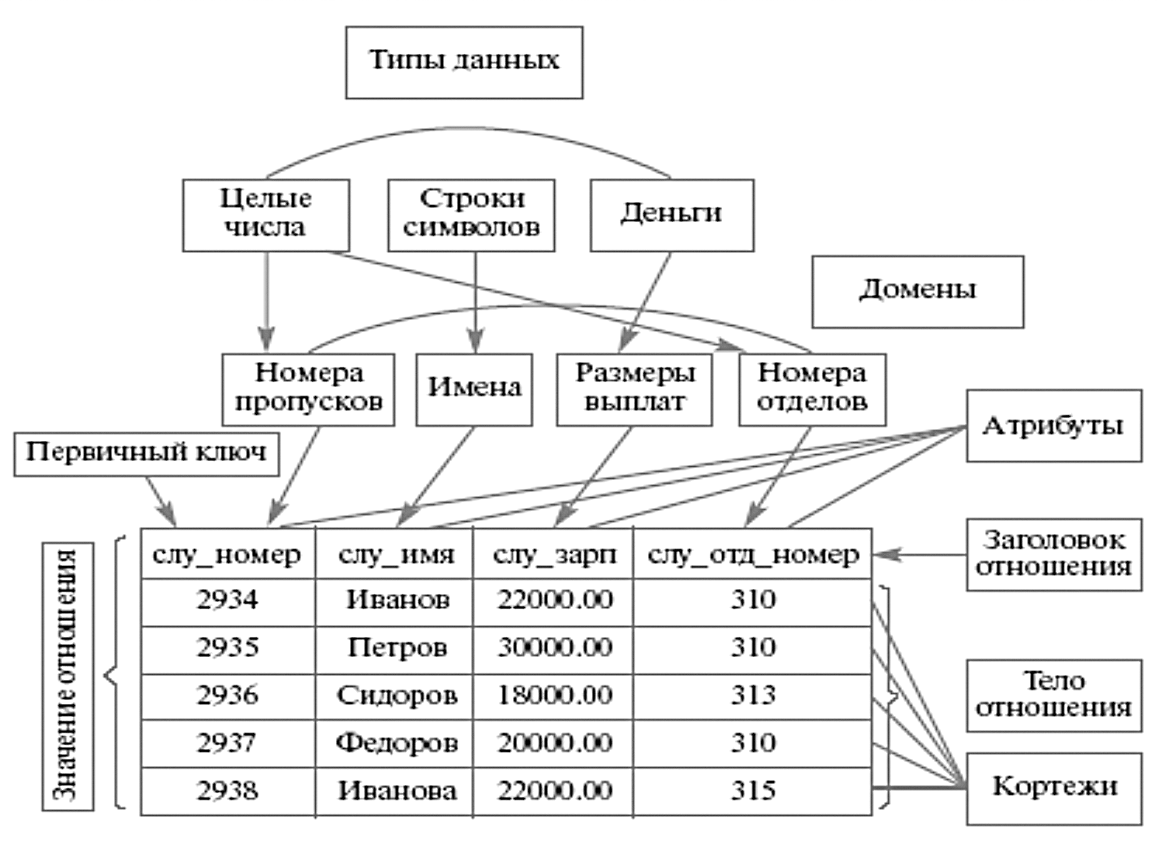
\includegraphics[scale=0.7]{./img/rel-model.png}
	\end{center}
	\caption{Основные понятия реляционной модели данных~\cite[c. 31]{Avrunyev2018}}
	\label{fig:rel-model}
\end{figure}

\textbf{Тип данных} в реляционной модели данных аналогичен типу данных в языках программирования и включает символы, числа, битовые строки, специализированные числовые данные (например, <<деньги>>) и <<темпоральные>> данные (дата, время).

\textbf{Домен} -- множество допустимых значений для типа данных. 

\textbf{Атрибут} -- некоторая характеристика объекта (сущности), имеющая уникальное имя внутри отношения, через которое к ниму производится обращение.

Атрибут, значение которого \textit{идентифицирует кортеж}, называется \textbf{ключом} отношения. В зависимости от количества атрибутов, входящих в ключ, различают простые и сложные (составные) ключи.

\textbf{Первичный ключ} -- уникальный атрибут (или их комбинация), который идентифицирует кортежи в таблице. Свойства: \textit{уникальность} (в любой момент времени никакие два кортежа отношения не должны иметь одно и то же значение); \textit{минимальность} (ни один из атрибутов не может быть исключен из набора атрибутов первичного ключа без нарушения свойств уникальности). 

В любой из таблиц может оказаться несколько наборов атрибутов, которые можно выбрать в качестве ключа, такие наборы называются \textbf{потенциальными} и \textbf{возможными} ключами.

\textbf{Внешний ключ} -- атрибут, который ссылается на первичный ключ другого отношения, обеспечивая связь между таблицами.

\textbf{Кортеж} -- это совокупность значений, где каждое значение (или элемент) соответствует определенному атрибуту, и эти значения принадлежат соответствующему домену атрибута.

Множество всех кортежей образует \textbf{отношение}, которое является подмножеством декартового произведения доменов, причем количество кортежей в отношении называется \textit{мощностью отношения}.

\textbf{Схема отношения (заголовок отношения)} -- набор упорядоченных пар <A, T>, где A -- имя атрибута, а T -- домен. Количество атрибутов в схеме называется \textit{степенью отношения}.

\textbf{Базовое отношение} -- содержит атрибуты и первичный ключ, а \textbf{производное отношение} -- используется для связи между таблицами.

Таким образом,  \textbf{реляционная база данных} -- это множество отношений, представленных в виде таблиц, где заголовок -- схема отношения, а строки -- кортежи.

\textbf{Фундаментальные свойства отношений}:
 \begin{enumerate}[label=---]
 	\item отсутствие кортежей-дубликатов;
 	\item отсутствие упорядоченности кортежей;
 	\item отсутствие упорядоченности атрибутов;
 	\item атомарность значений атрибутов (является базовым требованием для реляционных баз данных -- требование нормализованных отношений или отношений, представленных в первой нормальной форме).
 \end{enumerate}

Реляционная модель данных, по К. Дейту, состоит из трех частей.
 \begin{enumerate}[label=\arabic*.]
 		\item  \textbf{Структурная часть} -- описывает организацию данных, включая таблицы (отношения), атрибуты и их типы, а также связи между таблицами.
 		\item \textbf{Манипуляционная часть} -- включает операции над данными, такие как выборка, добавление, обновление и удаление данных, что осуществляется через язык запросов (например, SQL).
 		\item \textbf{Целостная часть} -- обеспечивает соблюдение целостности данных, включая ограничения (например, уникальность значений, ссылки между таблицами через внешние ключи), чтобы поддерживать корректность и непротиворечивость данных в базе~\cite[С. 30-35]{Avrunyev2018}.
 \end{enumerate}
 
 \subsubsection{Модель данных <<ключ-значение>>}
 
 \textbf{Модель данных ключ-значение} представляет собой структуру данных, которая использует ассоциативный массив, где каждый элемент состоит из \textit{уникального ключа} и \textit{связанного с ним значения}. Значение может быть любым типом данных, но оно не имеет структуры.
 
 Эта модель поддерживает \textbf{две основные операции}:
  \begin{enumerate}[label=---]
  	\item \textbf{получение значения по ключу} -- если ключ существует, возвращается связанное с ним значение, иначе -- NULL (специальное значение, которое используется в базах данных для обозначения отсутствия данных или неизвестного значения).
  	\item \textbf{запись значения по ключу} -- позволяет добавить или обновить значение для определенного ключа (также возможно установить время жизни ключа, после чего он будет автоматически удален) ~\cite[С. 89-91]{Avrunyev2018}.
  \end{enumerate}

 
\subsubsection{Документная модель данных}

Модель документная расширяет представление модели <<ключ-значение>>, позволяя хранить более сложные структуры данных -- документы.

\textbf{Документная модель данных} -- это подход к организации и хранению данных, при котором данные представлены в виде документов.

\textbf{Основные характеристики документной модели}:
 \begin{enumerate}[label=\arabic*)]
	\item документ как основная единица хранения;
	\item \textbf{документ} -- это структурированный набор данных, который может содержать различные пары \textit{ключ-значение} и может включать
	\begin{enumerate}[label=---]
		\item простые типы данных: строки, числа, булевы значения;
		\item упорядоченные списки значений;
		\item вложенные документы: другие объекты, которые могут быть представлены в формате пары ключ-значение;
		\item сложные типы данных: например, даты, бинарные данные и другие;
	\end{enumerate}
	\item отсутствие операций соединения -- cвязанные данные обычно хранятся в одном документе~\cite[С. 92-96]{Avrunyev2018}.
\end{enumerate}

\subsubsection*{Выбор модели данных}

Для базы данных фитнес-клуба была выбрана реляционная модель данных, поскольку она наиболее подходит для работы с хорошо структурированными данными и поддерживает сложные связи между сущностями, такими как клиенты, тренеры, абонементы и расписания. 

Для кэширования данных была выбрана модель <<ключ-значение>>, так как она подходит для быстрого доступа к данным, часто запрашиваемым пользователями, таким как актуальные типы абонементов или специализации тренеров, которые не требуют хранения сложного структурированного набора данных, например, документов. 

\subsection{Обзор существующих решений}

\subsubsection*{1С:Фитнес клуб}

\textbf{1С:Фитнес клуб} -- это программное решение для автоматизации фитнес-клубов и спортивных учреждений, созданное компанией <<Лаборатория программного обеспечения>>. 

\begin{figure}[ht!]
	\begin{center}
		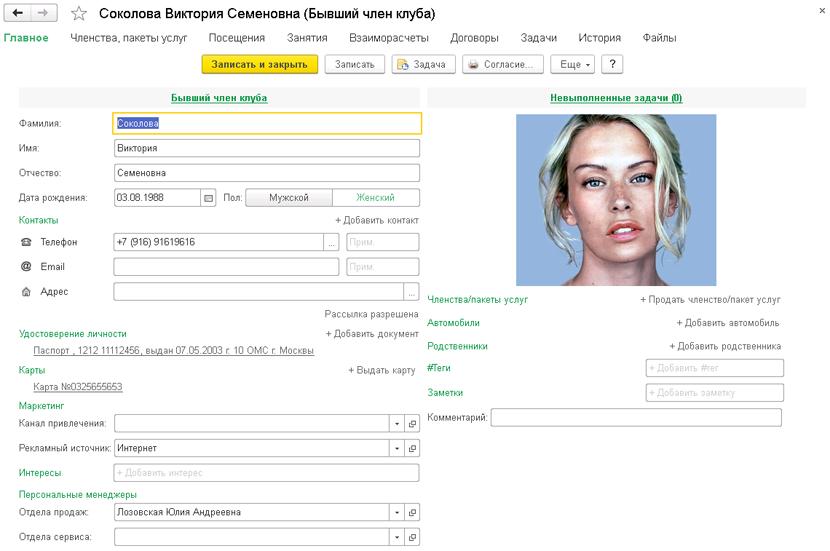
\includegraphics[scale=0.46]{./img/1c-1.png}
	\end{center}
	\caption{Интерфейс администратора для управления данными клиента фитнес-клуба приложения 1C:Фитнес клуб}
	\label{fig:1c-1}
\end{figure}

Приложение включает в себя функционал для работы с клиентской базой, маркетинга, расчета заработной платы, учета посещений, CRM-систему, интеграции с внешними сервисами и мобильные приложения для персонала. 

\begin{figure}[ht!]
	\begin{center}
		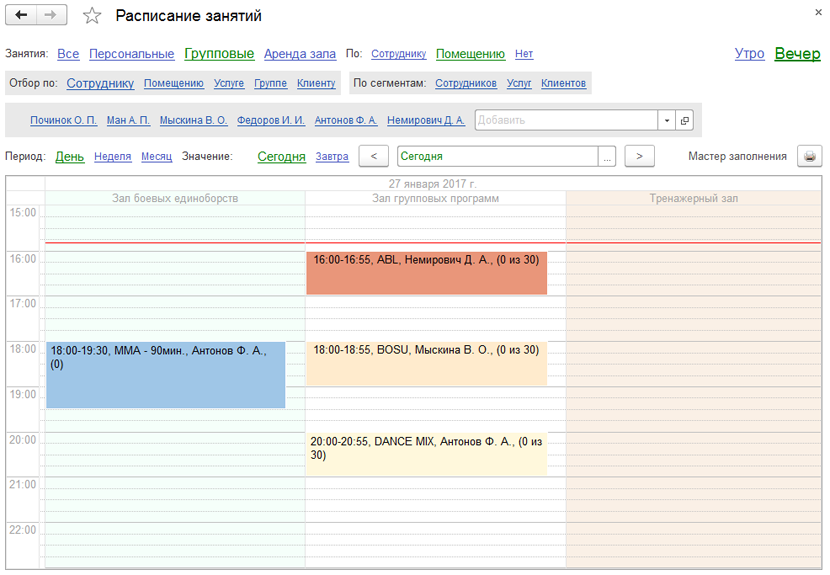
\includegraphics[scale=0.46]{./img/1c-2.png}
	\end{center}
	\caption{Интерфейс администратора для управления расписание тренировок фитнес-клуба приложения 1C:Фитнес клуб}
	\label{fig:1c-2}
\end{figure}

Приложение не предоставляет пробный период, но предлагает несколько тарифных планов, подходящих для разных масштабов бизнеса. Тарифы варьируются от 1 990 рублей в месяц за облачную подписку с базовым набором функций до 90 000 рублей за покупку программы с расширенными возможностями.

Для работы приложения необходима операционная система Windows. Для онлайн версии требуется постоянный интернет на компьютере.

\subsubsection*{fitness365}

\textbf{fitness365} -- это веб-система, специально разработанная для комплексного управления фитнес-клубом. Она предоставляет широкий набор инструментов, которые охватывают все аспекты работы клуба: от работы с клиентами до ведения статистики и аналитики.

fitness365 имеет интегрированную CRM-систему, которая позволяет клубу управлять базой клиентов -- каждому пользователю предоставляется персонализированный доступ.

\begin{figure}[ht!]
	\begin{center}
		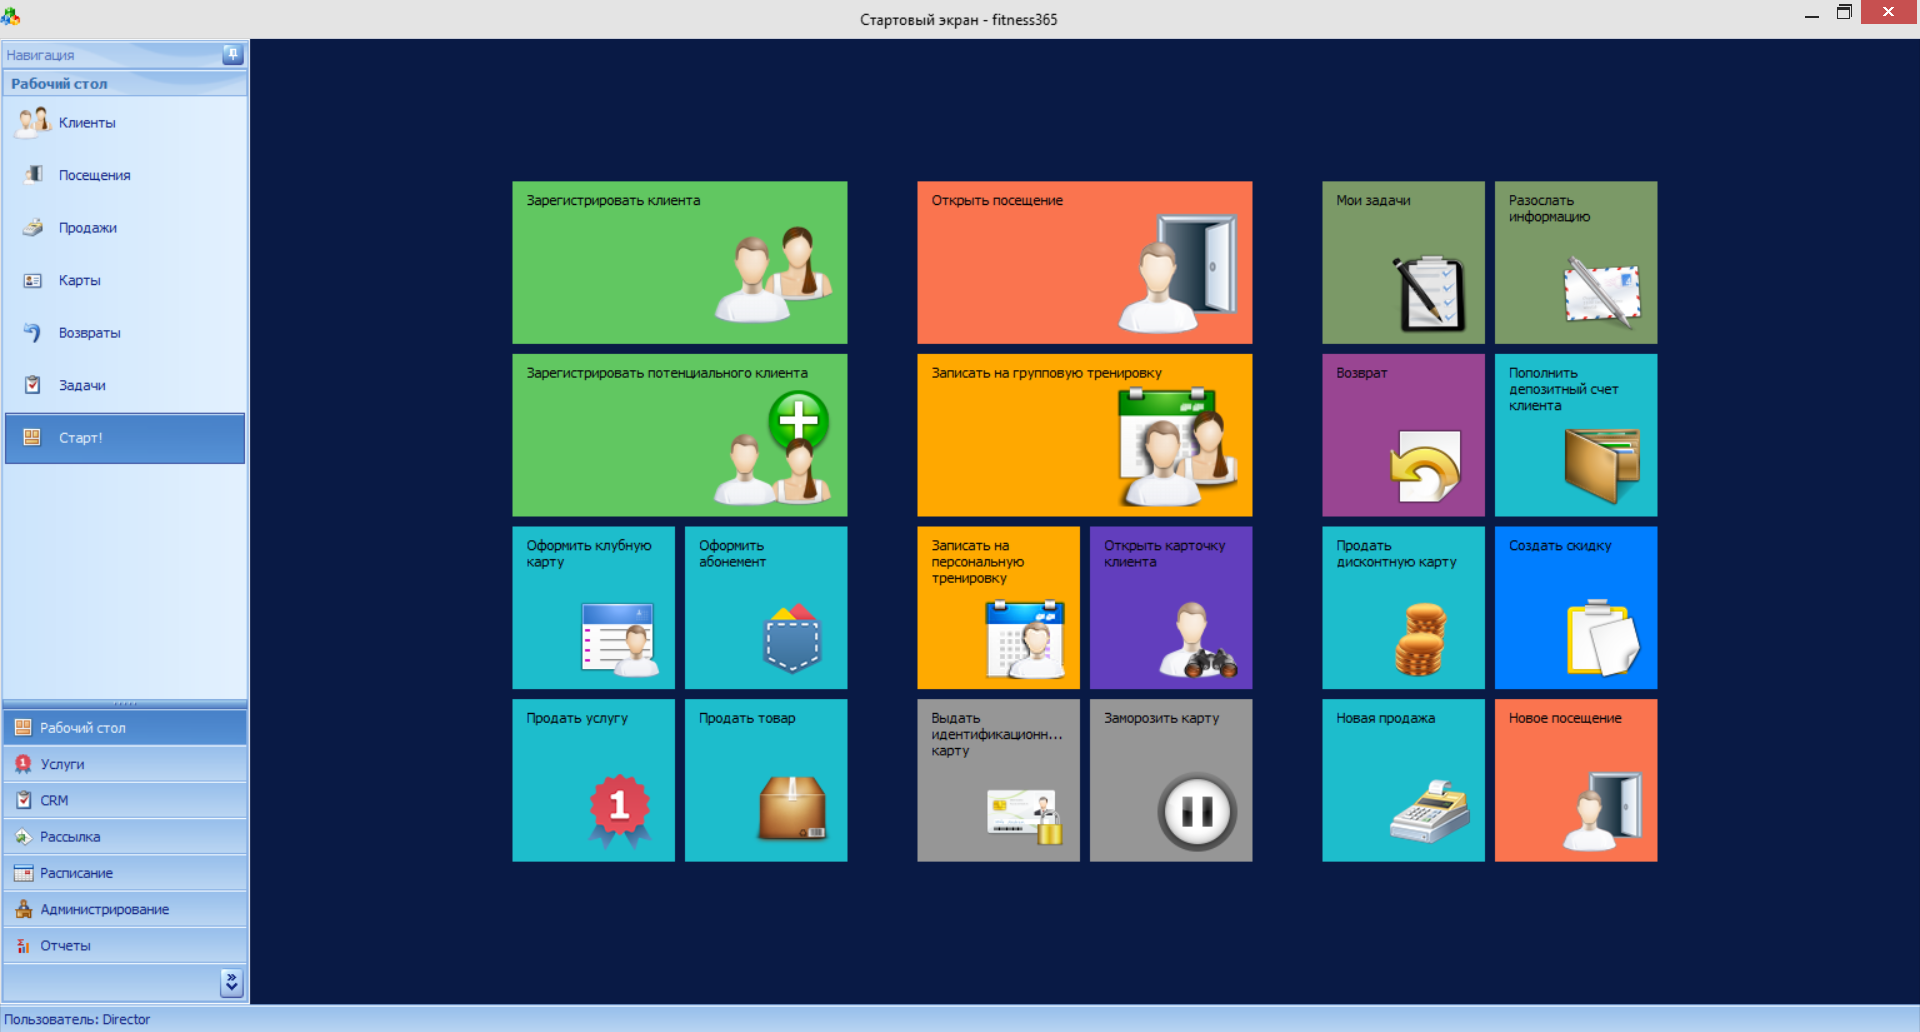
\includegraphics[scale=0.35]{./img/f365-1.png}
	\end{center}
	\caption{Интерфейс главной страницы администратора фитнес-клуба приложения fitness365}
	\label{fig:f365-1}
\end{figure}

\begin{figure}[ht!]
	\begin{center}
		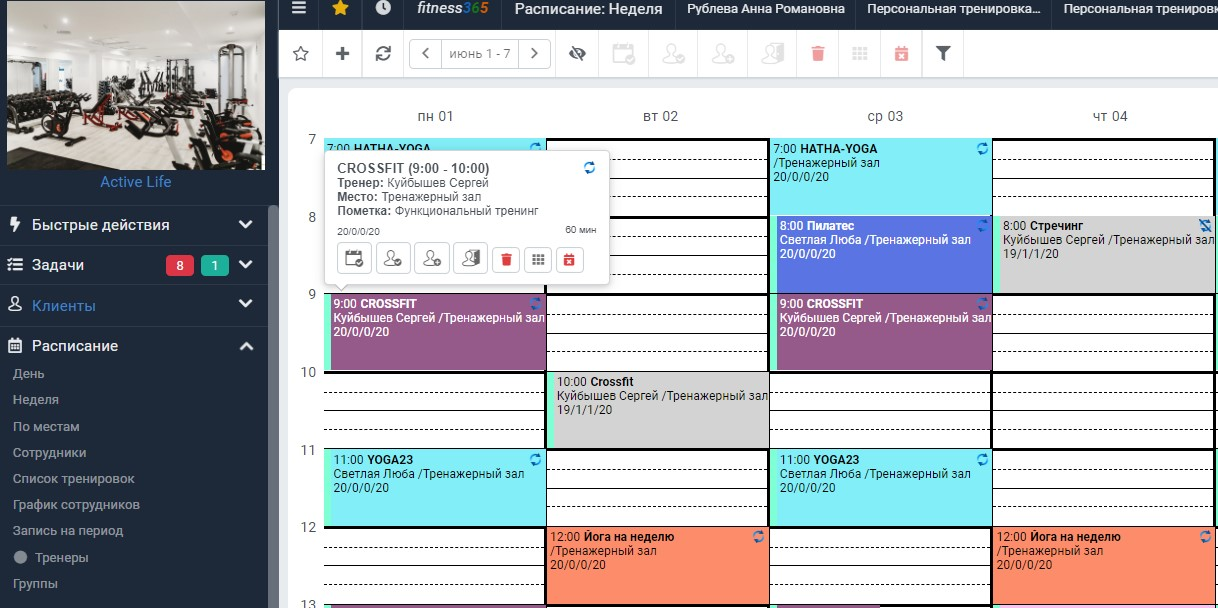
\includegraphics[scale=0.45]{./img/f365-2.png}
	\end{center}
	\caption{Интерфейс администратора для управления расписанием фитнес-клуба приложения fitness365}
	\label{fig:f365-2}
\end{figure}

Тарифы fitness365 предлагают различные опции для фитнес-клубов. Например, тариф <<Онлайн>> стоит 2 000 рублей в месяц, включает доступ через интернет и возможность работы с неограниченным числом клиентов, но поддерживает 5 рабочих мест. Для клубов, где проблемы с интернетом, доступна настольная версия за разовый платеж 44 000 рублей. Кроме того, есть дополнительные опции за дополнительную оплату.

Для работы приложения необходима операционная система Windows. Для онлайн версии требуется постоянный интернет на компьютере.

\subsubsection*{Сравнение решений}

\begin{table}[ht]
	\centering
	\begin{tabular}{|p{9cm}|c|c|}
		\hline
		\textbf{Функциональность для администратора} & \textbf{1С:Фитнес Клуб} & \textbf{fitness365} \\ \hline
		Управление расписанием, залами и персоналом & + & + \\ \hline
		Работа с абонементами и услугами & + & + \\ \hline
		Ведение клиентской базы и CRM & + & + \\ \hline
	\end{tabular}
	\begin{tabular}{|p{9cm}|c|c|}
		\hline
		\textbf{Функциональность для клиента} & \textbf{1С:Фитнес Клуб} & \textbf{fitness365} \\ \hline
		Наличие личного кабинета & + & + \\ \hline
		Покупка абонементов онлайн & + & + \\ \hline
		Самостоятельная запись на тренировки & + & + \\ \hline
	\end{tabular}
	\begin{tabular}{|p{9cm}|c|c|}
		\hline
		\textbf{Функциональность для тренера} & \textbf{1С:Фитнес Клуб} & \textbf{fitness365} \\ \hline
		Доступ к информации о клиентах & -- & + \\ \hline
		Просмотр и управление своим расписанием & -- & -- \\ \hline
		Мобильный доступ к системе & -- & -- \\ \hline
	\end{tabular}
	\caption{Сравнение функциональности по 1С:Фитнес Клуб и fitness365}
\end{table}

Рассматриваемые решения, такие как 1С:Фитнес Клуб и fitness365, могут быть избыточными для конкретных нужд фитнес-клуба, что делает их сложными и громоздкими для использования в условиях небольших или специализированных клубов. Также они ориентированы на платформу Windows и предлагают доступ через интернет, что ограничивает их использование преимущественно стационарными компьютерами -- это может быть неудобно для тренеров и клиентов, которым необходим постоянный доступ к системе, особенно в условиях мобильности. Кроме того, все рассматриваемые решения являются достаточно дорогими, что может стать препятствием для небольших фитнес-клубов. 

Мобильные устройства позволяют обеспечить доступ к системе в любом месте и в любое время, поэтому разрабатываемое приложение для доступа к базе данных будет мобильным, ориентированным на платформу iOS. Также приложение будет сфокусировано на ключевых функциях, таких как управление расписанием для тренеров и клиентов, самостоятельный контроль личного кабинета. Кроме того, приложение будет бесплатным, что делает его более доступным для широкого круга пользователей. 

\subsection*{Вывод}

В данном разделе проведен анализ предметной области фитнес-клубов, описана структура базы данных, рассмотрены пользователи базы данных и их права доступа. Также проведен анализ различных моделей данных, в результате чего для хранения данных выбрана реляционная модель данных, а для кэширования -- модель <<ключ-значение>>. Рассмотрены существующие решения и их особенности.
